\documentclass[oneside,hidelinks]{book}

\usepackage[english]{babel}
\usepackage[utf8x]{inputenc}
\usepackage{amsmath}
\usepackage{amsfonts}
\usepackage{amssymb}
\usepackage{graphicx}
\usepackage{hyperref}
\usepackage{color}
\usepackage{subfiles}
\usepackage{caption}
\usepackage{listings}
\usepackage{color}
\usepackage{xcolor}
\usepackage{courier}
\usepackage{geometry}
\usepackage{tikz}							% graph theory
\lstset{ %
language=Python,							% choose the language of the code
basicstyle=\footnotesize\ttfamily,			% the size of the fonts that are used for the code
%basicstyle=\footnotesize,			% the size of the fonts that are used for the code
numbers=left,								% where to put the line-numbers
numberstyle=\footnotesize,					% the size of the fonts that are used for the line-numbers
stepnumber=1,								% the step between two line-numbers. If it is 1 each line will be numbered
numbersep=10pt,								% how far the line-numbers are from the code
backgroundcolor=\color{red!2},				% choose the background color. You must add \usepackage{color}
showspaces=false,							% show spaces adding particular underscores
showstringspaces=false,						% underline spaces within strings
showtabs=false,								% show tabs within strings adding particular underscores
frame=single,								% adds a frame around the code
tabsize=4,									% sets default tabsize to 2 spaces
captionpos=b,								% sets the caption-position to bottom
breaklines=true,							% sets automatic line breaking
breakatwhitespace=false,					% sets if automatic breaks should only happen at whitespace
escapeinside={\%*}{*)}						% if you want to add a comment within your code
}
\captionsetup[lstlisting]{labelformat=empty}
\captionsetup[figure]{labelformat=empty}

\usepackage{enumitem}
\setitemize{itemsep=2px}

\begin{document}

\thispagestyle{empty}

\newgeometry{top=0mm, bottom=0mm}

~
\vspace{129px}

\begin{center}
{\Huge \textbf{Source}}\\
\vspace{10px}
{\textit{An infinite game...}}\\
\end{center}

\vspace{129px}

\begin{center}
  \makebox[\textwidth]{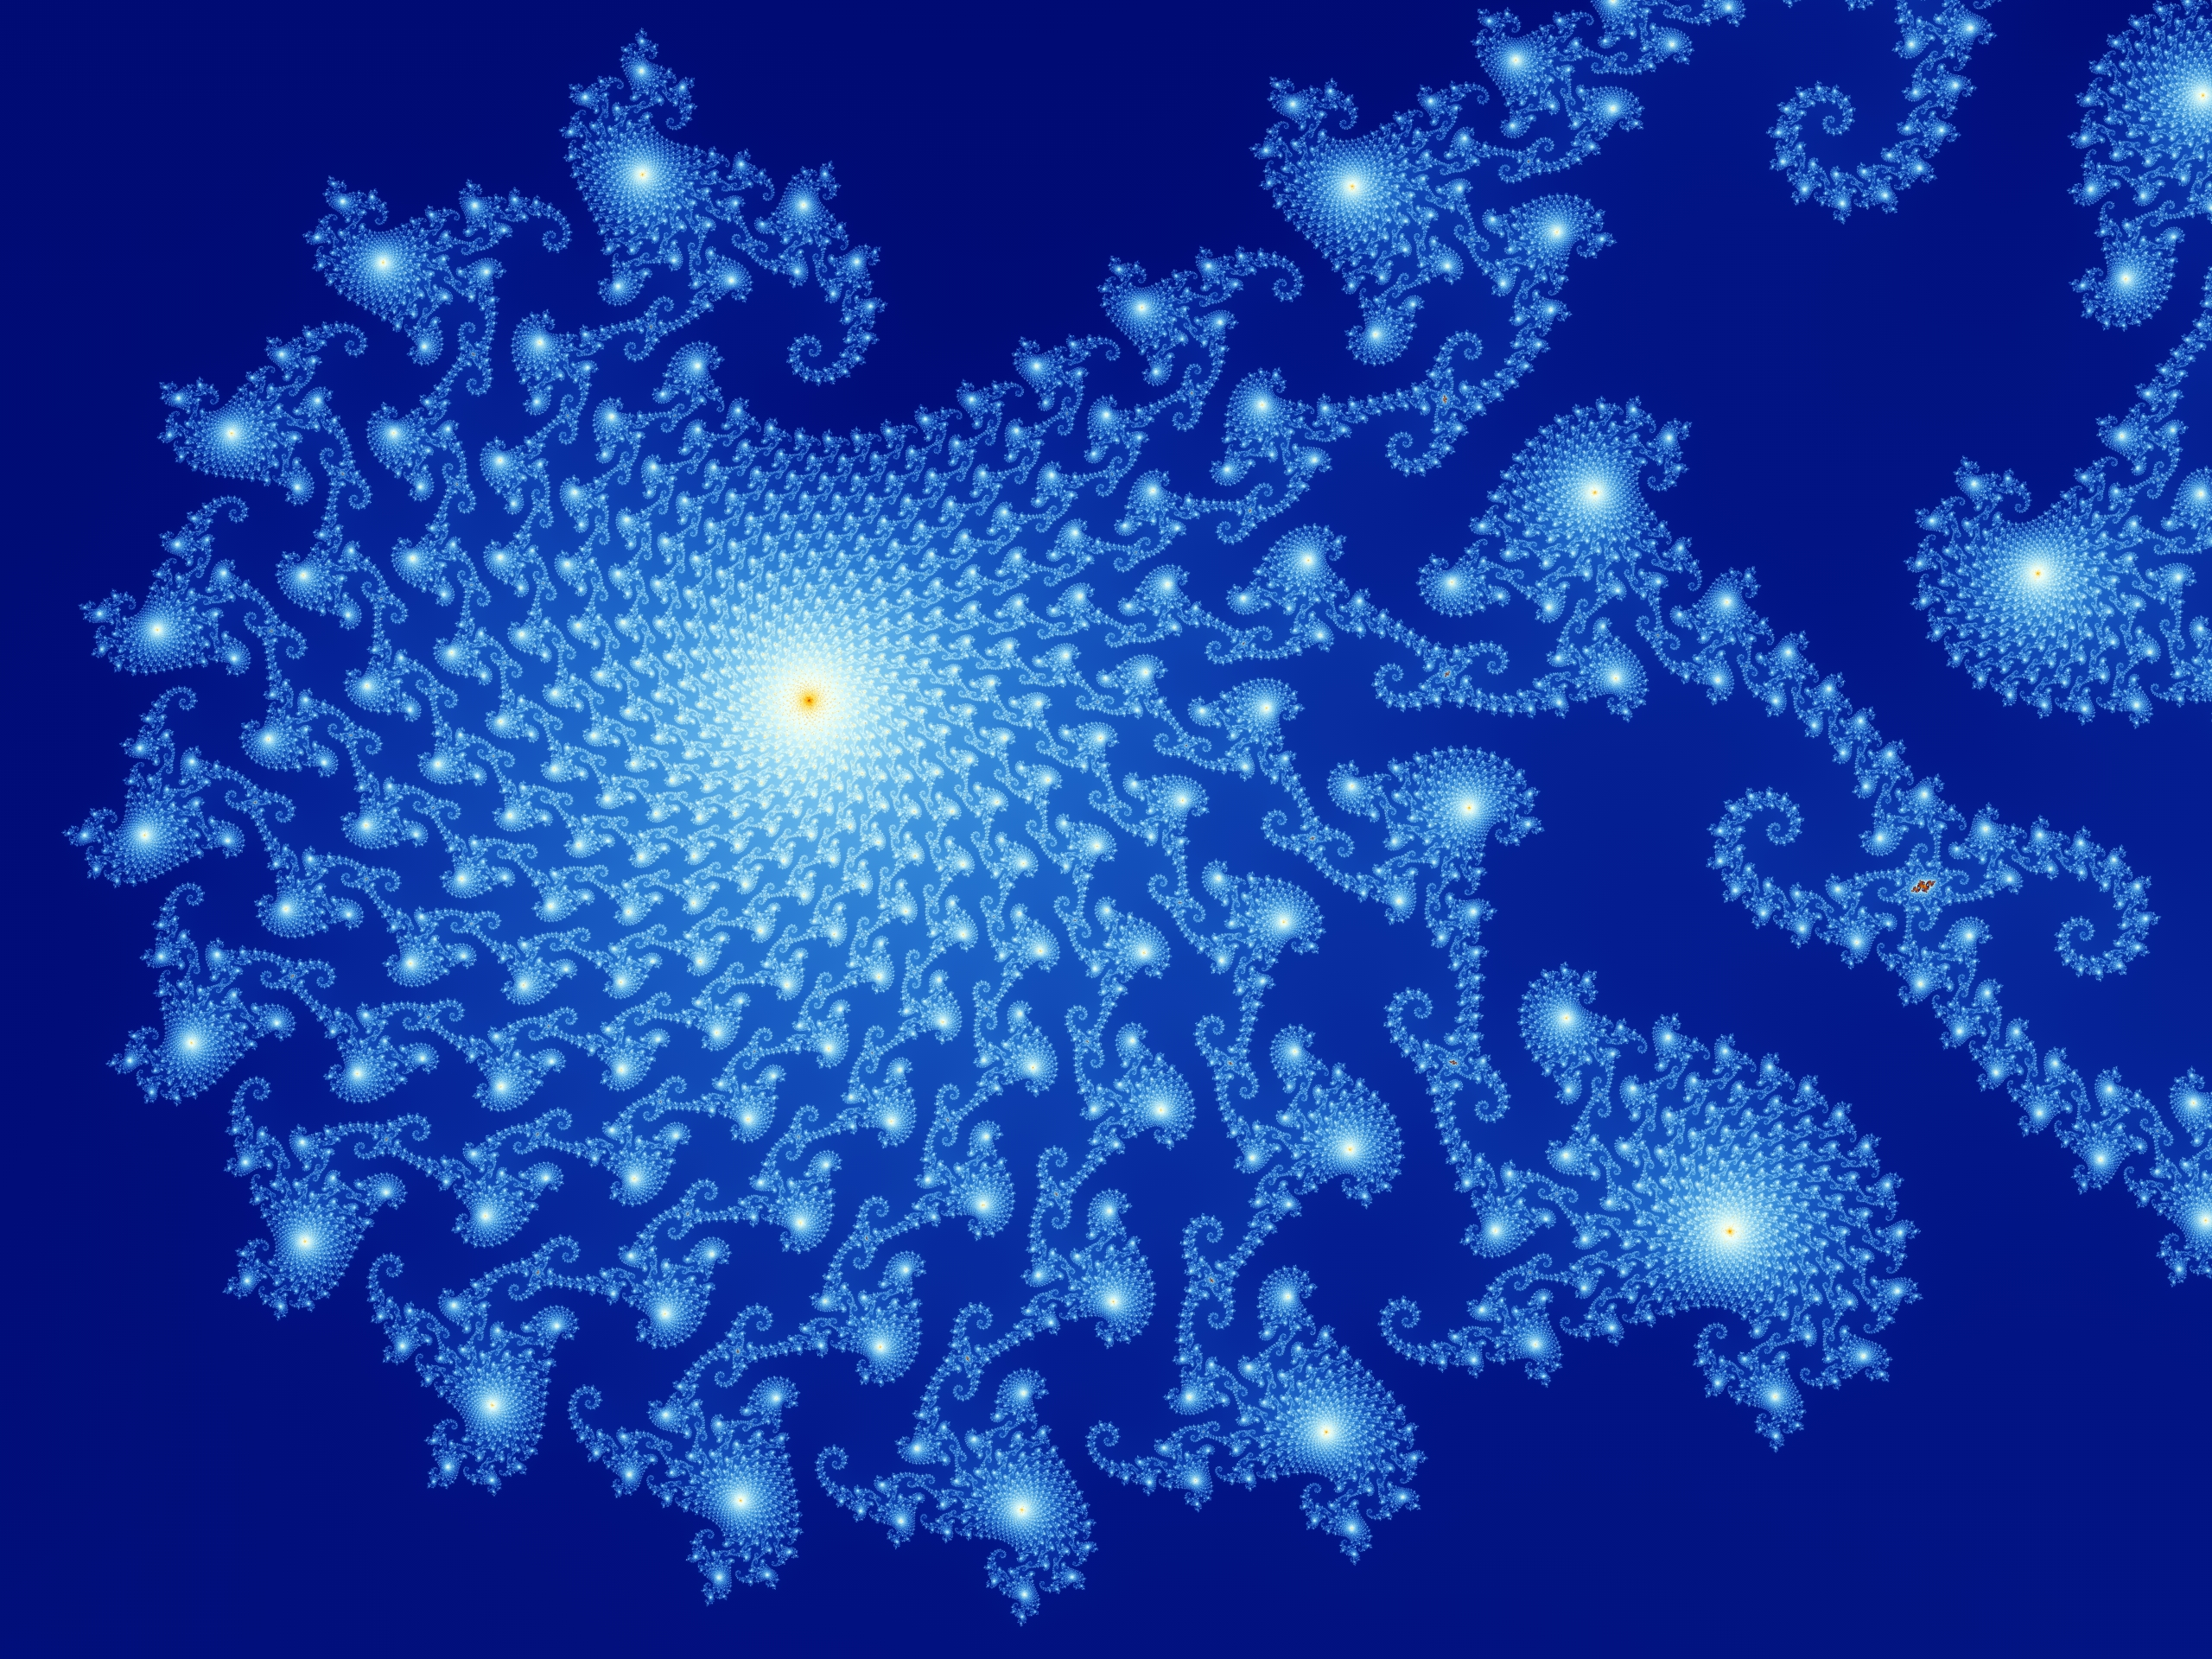
\includegraphics[width=620px]{images/mandel_zoom.jpg}}
\end{center}

\newpage

\restoregeometry

\newgeometry{margin=1.5in}

\thispagestyle{empty}

\vspace{20px}

\textbf{License} \\
Permission is granted to copy, distribute and/or modify everything in this document under the terms of the Creative Commons Attribution-ShareAlike 4.0 International License.\\

\textbf{References} \\
References to external works are in a separate file: \href{https://github.com/rjelavic/hello-world/blob/master/bibliography.md}{\texttt{bibliography.md}}\\

\textbf{Images}\\
The following images are not under public domain:
\begin{itemize}
\item \textbf{Page 1} - \url{https://commons.wikimedia.org/wiki/File:Mandel_zoom_12_satellite_spirally_wheel_with_julia_islands.jpg}
\end{itemize}

\tableofcontents

\part{Ontology}

\chapter{Knowledge}

\subfile{lib/knowledge}

\chapter{States}

\chapter{Interference}

\part{Complexity}

\chapter{Patterns}

\chapter{Optimization}

\chapter{Replication}

\part{Action}

\chapter{Agents}

\chapter{Exchange}

\chapter{Coordination}

\part{Meta}

\chapter{Thought}

\chapter{Introspection}

\chapter{Structure}

\end{document}
